This example illustrate performances of particle filter to highly non-linear filter. The promblem here involves a plane whose the trajectory is a brownian motion. This aircraft measure the elevation. The measure of this elevation and an elevation map are then used to estimate the position of the plane.  \begin{ImageNoCaption}\mbox{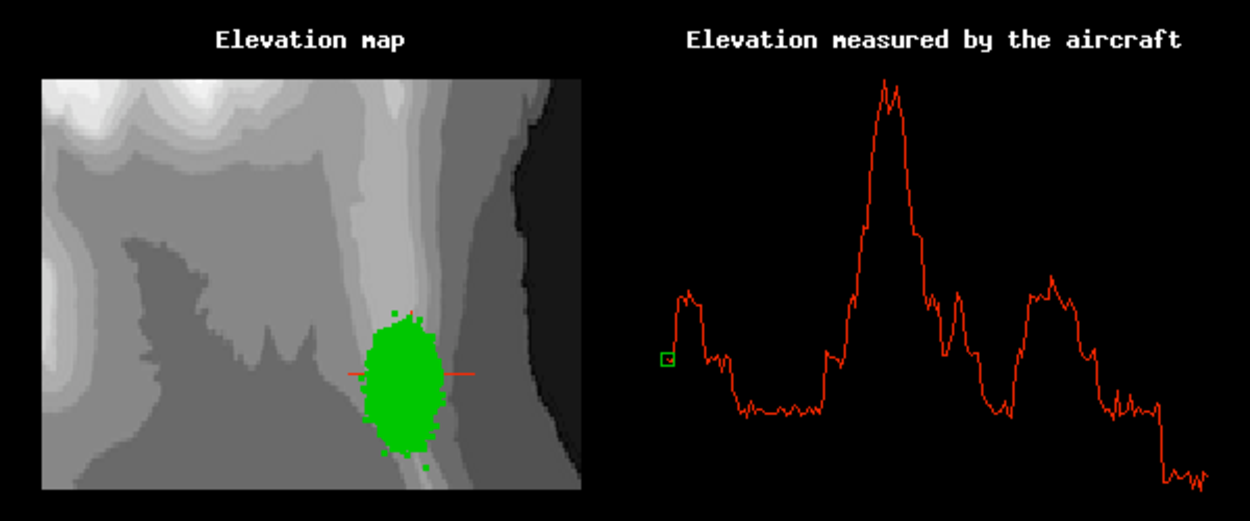
\includegraphics{plane}}
\end{ImageNoCaption}


plane.h 

\begin{DocInclude}\begin{verbatim}#ifndef __PLANE
#define __PLANE

#include <bfilt/gaussian_model.h>

class Plane : public Gaussian_Nonlinear_Model
{
      vector<double> Map;
      double xmin;
      double xmax;
      double ymin;
      double ymax;

      double sigv;
      double sigc;
public :
      Plane(const char *filename);

      dcovector State_Function(const dcovector &X, const dcovector &W);
      dcovector Observation_Function(const dcovector & X);
};


#endif
\end{verbatim}
\end{DocInclude}
 plane.cpp 

\begin{DocInclude}\begin{verbatim}#include "plane.h"

Plane::Plane(const char * filename)
{
      int x,y,z;
      ifstream file(filename);

      if(file)
            {
                              file>>xmax;
                              file>>ymin;
                              file>>z;
                              Map.push_back(z);

                  while(!file.eof())
                        {
                              file>>x;
                              file>>y;
                              file>>z;
                              Map.push_back(z);

                              if(x>xmax)
                                    xmax=x;
                              if(x<xmin)
                                    xmin=x;
                              if(y>ymax)
                                    ymax=y;
                              if(y<ymin)
                                    ymin=y;
                              
                        }
                  file.close();
            }
      else 
            {
                  cout<<"Plane :: error file"<<endl;
            }

      Qw.resize(2);
      Qw.identity();
      Qv.resize(1);
      Qv.identity();
      Qv*=5.;
      R0.resize(4);
      R0.zero();
      R0(0,0)=10.;
      R0(1,1)=10.;
      R0(2,2) = .001;
      R0(3,3) = 0.0001;
      X0.resize(4);
      X0(0)=120.;
      X0(1)=20.;
      X0(2)=1.5;
      X0(3)=2.35;


      sigv = .001;
      sigc = 0.03;
            
}

dcovector Plane::State_Function(const dcovector &X, const dcovector &W)
{
      dcovector U(4);

      U(0) = X(0) + X(2) * cos(X(3));
      U(1) = X(1) + X(2) * sin(X(3));
      U(2) = X(2) + sigv * W(0);
      U(3) = X(3) + sigc * W(1);
      if (U(0)>xmax)
            {
                  U(0)=xmax;
                  U(3)=3.14-U(3);
            }
      if (U(1)>ymax)
            {
                  U(1)=ymax;
                  U(3)=-U(3);
            }
      if (U(0)<xmin)
            {
                  U(0)=xmin;
                  U(3)=3.14-U(3);
            }
      if (U(1)<ymin)
            {
                  U(1)=ymin;
                  U(3)=-U(3);
            }

      return U;
}
dcovector Plane::Observation_Function(const dcovector & X)
{
      int x = (int)(X(0));
      int y = (int)(X(1));
      int j= (xmax+1)*y + x;
      dcovector Y(1);
      Y(0)=Map[j];
      return Y;
}

\end{verbatim}
\end{DocInclude}
 The main program : 

\begin{DocInclude}\begin{verbatim}#include <bfilt/simulator.h>
#include <bfilt/sisr_filter.h>
#include "plane.h"

// This example illustrate performances of particle filter to highly non-linear 
// filter. The promblem here involves a plane whose the trajectory is a brownian
// motion. This aircraft measure the elevation. The measure of this elevation and 
// an elevation map are then used to estimate the position of the plane.
int main(int argc, char **argv)
{
      int k;
      int i;
      int j;
      vector<Weighted_Sample> cloud;

      ofstream file_c("../data/cloud.dat"); // To save the cloud
      ofstream file_s("../data/state.dat"); // To save the state

      Plane       plane("../data/map_2.dat");       // The plane model
      G_Simulator sim(&plane);                    // To simulate a this model
      
      Bootstrap_Filter filter(100000,&plane);       // A bootstrap filter to estimate the position

      sim.Simulate(150);                     // simulation of 250 samples

      sim.Save_Y("../data/output.dat");     // save the output

      // Here Init() and Update methods are used
      // for filtering because we want to get the cloud 
      // at each step and save it in cloud.dat

      filter.Init();                      // Initialization of the boostrap filter
      
      for (k=0; k<sim.Y.size(); k++)
            {

                  cloud=filter.CloudGet();              // The current cloud is return

                  for(i=0; i<cloud.size(); i++)         // and here it is saved
                        {
                              for(j=0; j<cloud[i].Value.l; j++)
                                    file_c<<cloud[i].Value(j)<<" ";
                              file_c<<endl;
                        }

                  for (j=0; j<sim.X[k].l; j++)       // The state is also saved
                        file_s<<sim.X[k](j)<<" ";
                  file_s<<endl<<endl<<endl;
                  file_c<<endl<<endl;

                  if( filter.Update(sim.Y[k]))              // The filter is then update with a new observation
                        filter.Init();
            }
      file_c.close();
      file_s.close();

      return 0;
}
\end{verbatim}
\end{DocInclude}
 